\chapter{Resultados}

En base al desempeño observado durante el desarrollo y prueba de cada una de las etapas de preprocesamiento, segmentación y clasificación, elegimos algunas de ellas para formar parte del algoritmo a evaluar. El algoritmo es (ver figura \ref{fig:esquemaalgoritmofinal}): 
%
\begin{enumerate}
\item Preprocesador: suavizado gaussiano
\item Segmentador: basado en imagen retroiluminada
\item Clasificador: según altura
\item Clasificador: según extensión de la caja envolvente
\item Clasificador: según relación de aspecto de los ejes de una elipse ajustada
\item Clasificador: según área sin tegumento (raspaduras) a partir de canales H, S y V
\item Clasificador: según media de color (canal H)
\item Clasificador: según desviación de color (canal H)
\item Clasificador: según media de color (canal a*)
\item Clasificador: según media de color (canal b*)
\item Clasificador: según solidez
\end{enumerate}

\begin{figure}[hbtp]
\centering
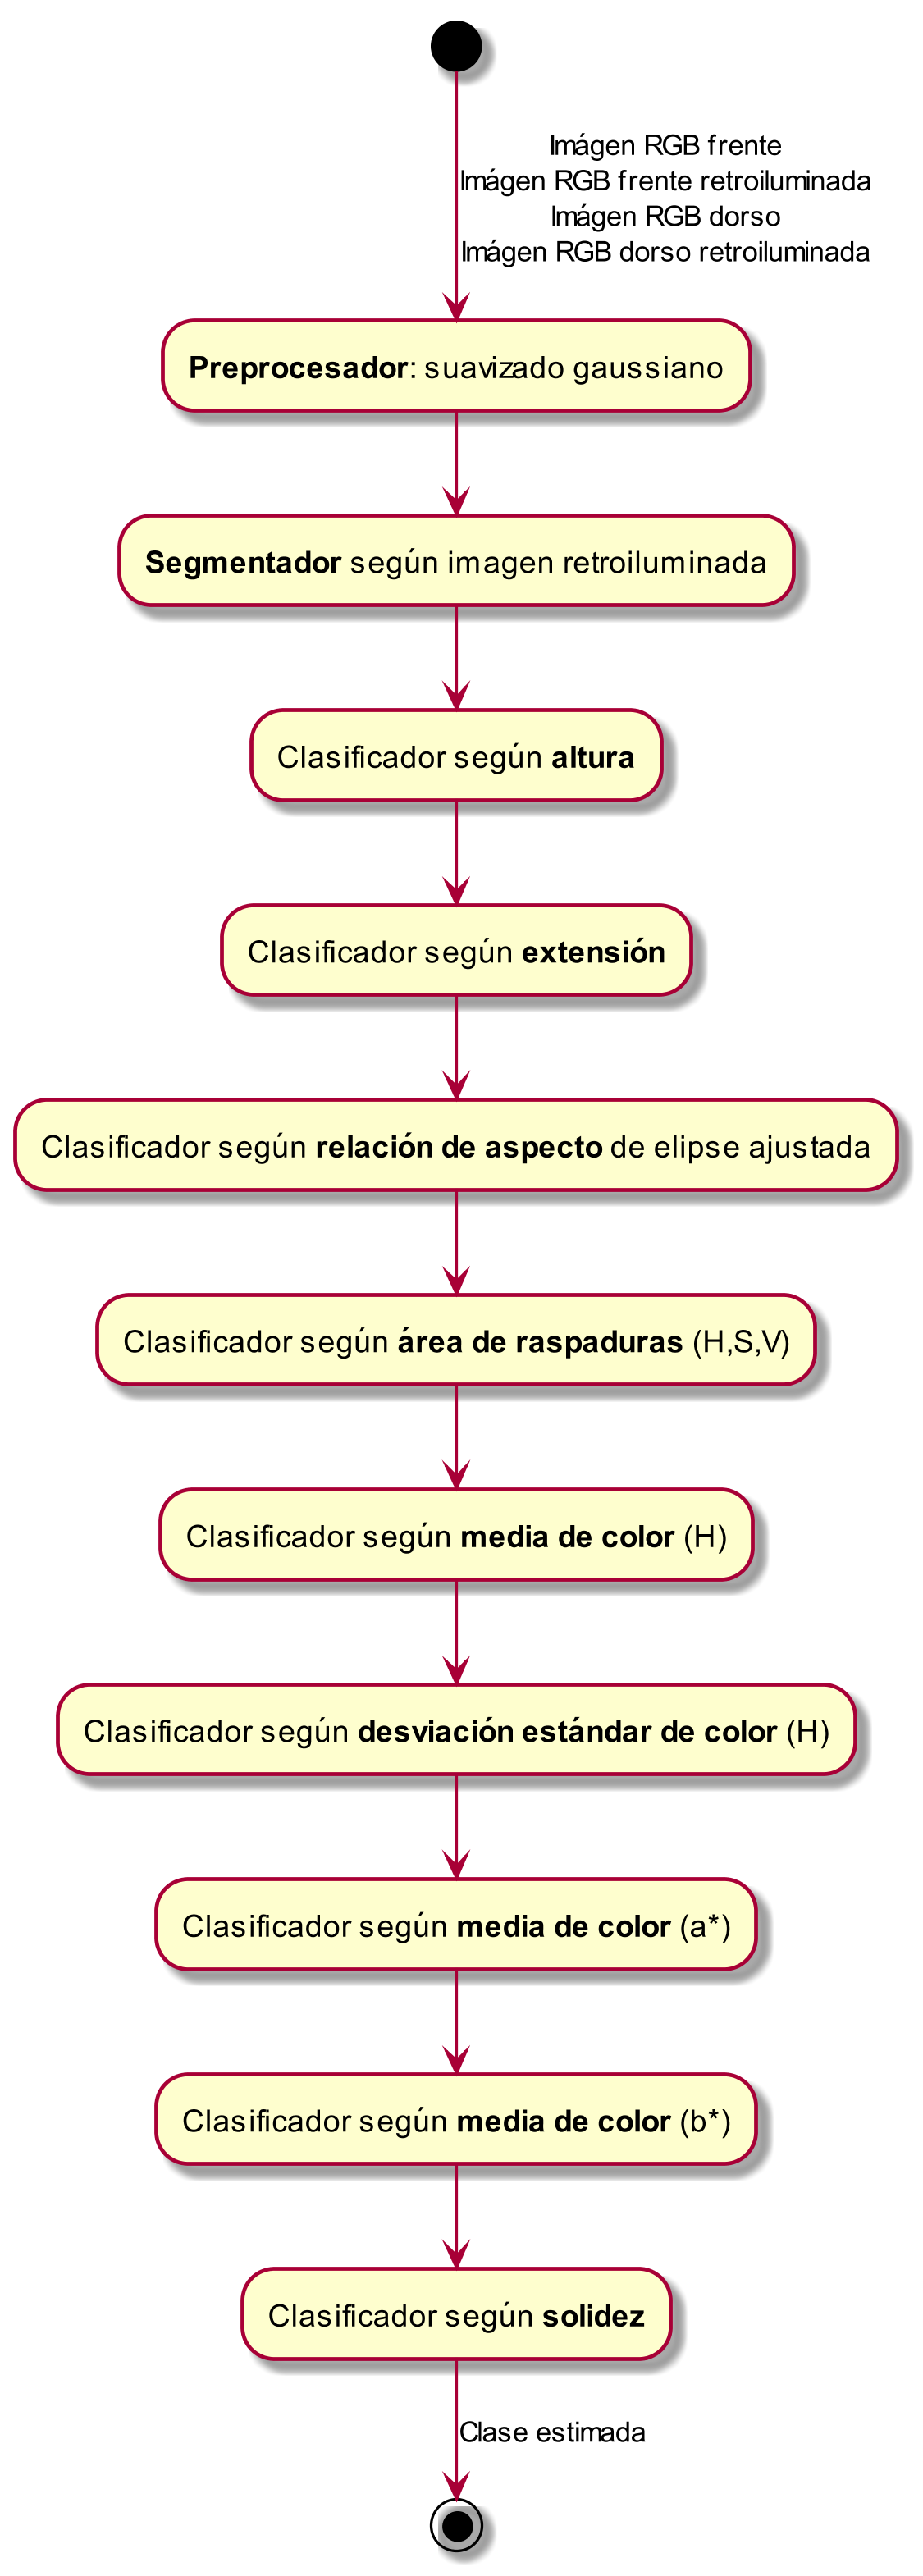
\includegraphics[width=\textwidth,height=0.9\textheight,keepaspectratio]{clasificadorfinal}
%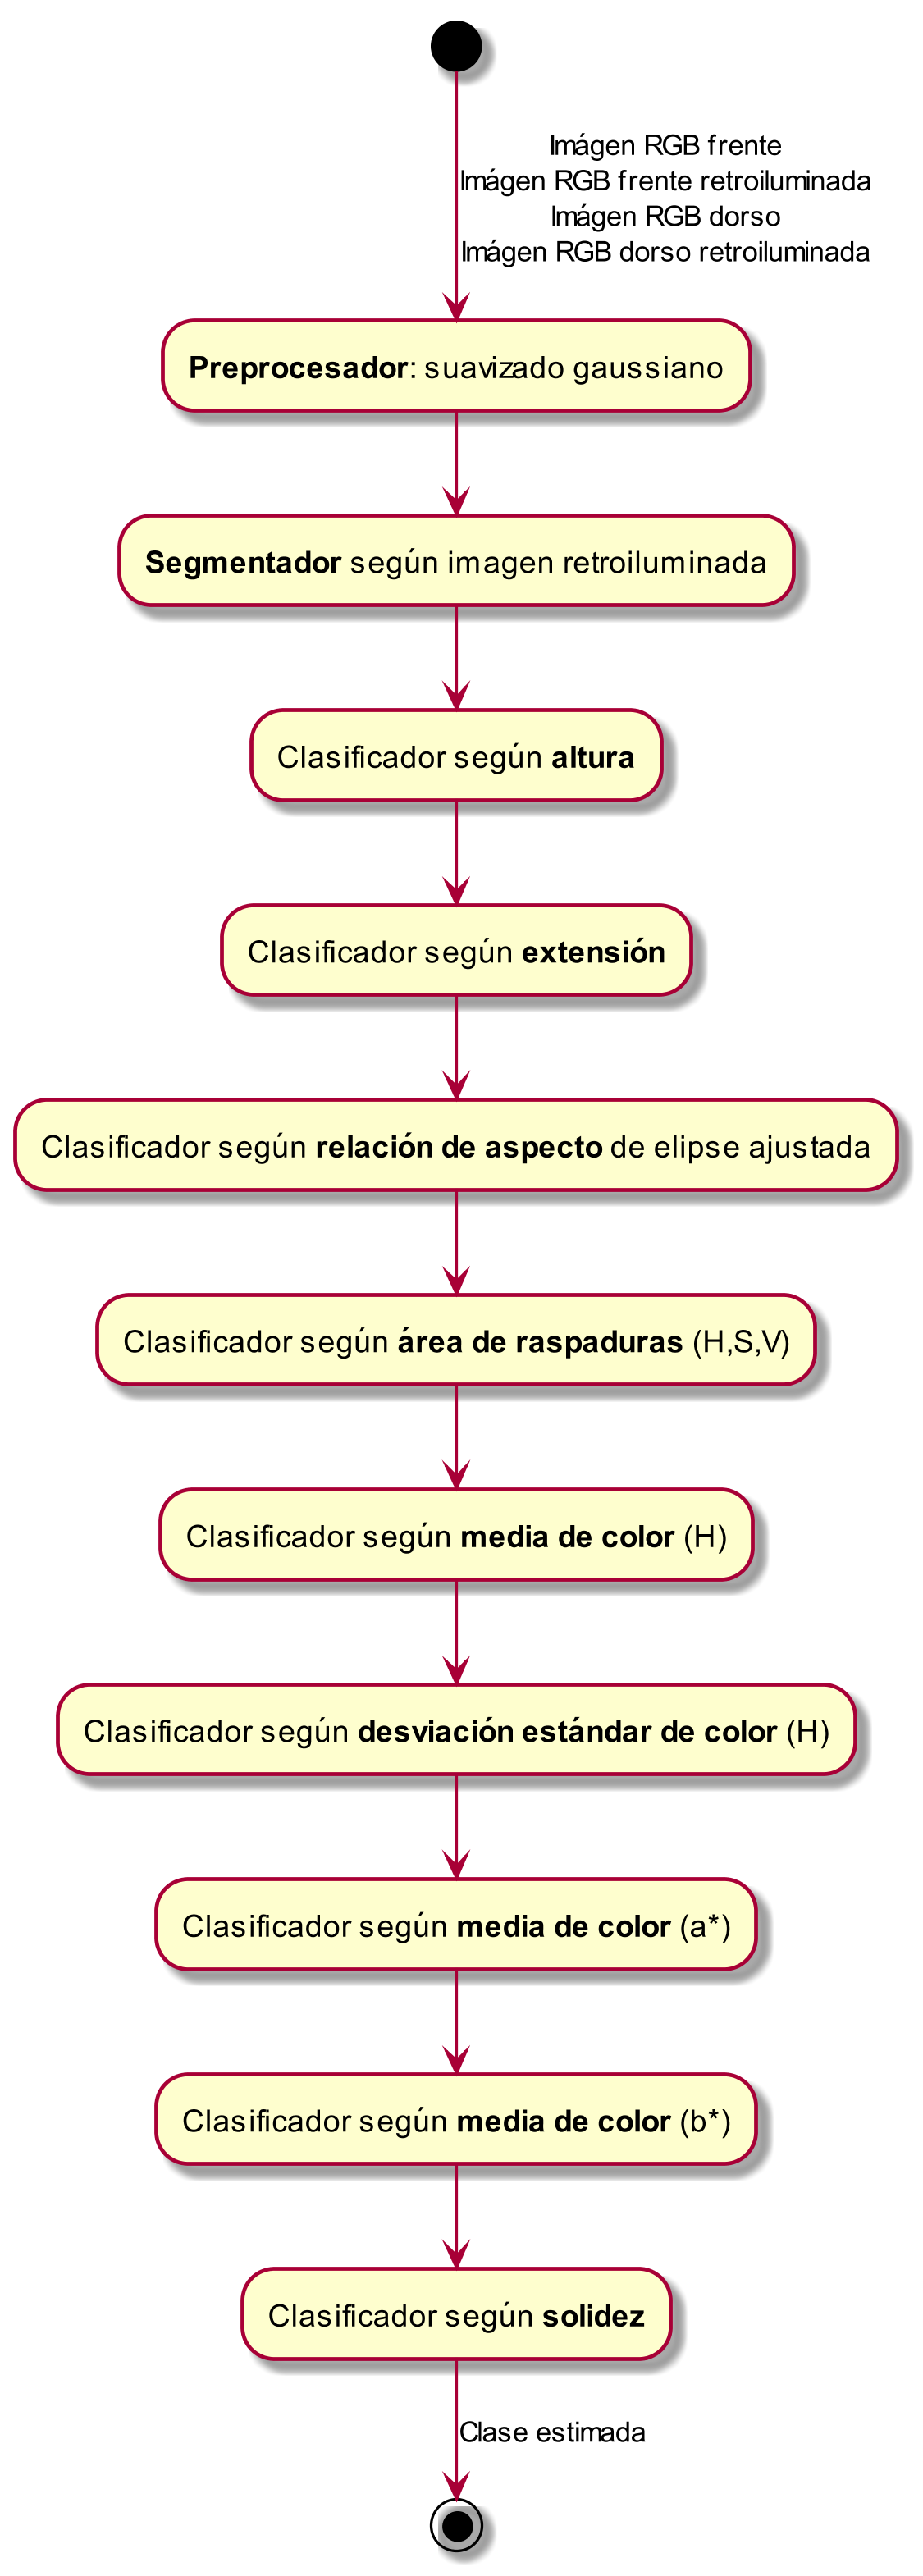
\includegraphics[scale=\escaladiagramas]{clasificadorfinal}
\caption[Etapas del algoritmo final]{etapas del algoritmo final.}
\label{fig:esquemaalgoritmofinal}
\end{figure}


Quedó fuera el clasificador según la relación de aspecto de la caja envolvente, porque es muy similar al de la relación de aspecto de la elipse ajustada. No se usó el clasificador según el área de arrugas por su mal desempeño general. El clasificador según área de raspaduras a partir de los canales H, S y V es mejor que el que solo usa S.

Es importante notar que los clasificadores según características de color (etapas \numlist{7;8;9;10}) realizan sus medidas a partir de los datos que están en las zonas con tegumento\footnote{También se pueden usar con la máscara del objeto completo.}; esta está determinada por la máscara creada por el clasificador según raspaduras y por tanto las medidas solo serán correctas en el caso de almendras y objetos de colores similares a los de las almendras.

Los parámetros de funcionamiento de cada clasificador fueron ajustados heurísticamente durante su desarrollo\footnote{Los valores se pueden ver en los archivos de clase correspondientes o en cualquier archivo \texttt{parametros\_efectivos*.yml} en las carpetas de experimentos.}, analizando su desempeño general o específico para el defecto que buscaban encontrar. Los parámetros que determinan los límites de clasificación se ajustarán según diferentes estrategias, como se menciona más adelante.





\section{Metodología de ajuste y evaluación}




\subsection{Evaluación}
La evaluación se hará sobre el conjunto \nombre{set3}, para dos casos de trabajo distintos:
\begin{enumerate}
\item Contemplando las tres clases del conjunto: Primera, Mala y No Almendra.
\item Simplificando a solo dos clases: Buena (clase Primera) y Mala (clase Mala y clase No Almendra). Esto se justifica porque no encontramos criterios confiables para separar las clases Mala y No Almendra.
\end{enumerate}

La evaluación se hará sobre el conjunto de evaluación —un \SI{20}{\percent} del total—, mientras que el ajuste de los parámetros de clasificación de cada etapa se hará según los valores de los descriptores sobre el conjunto de entrenamiento —el restante \SI{80}{\percent}—. Ver \ref{captura:particionypreprocesado}.

Los resultados de nuestro clasificador serán contrastados contra los obtenidos por algoritmos de aprendizaje automático en \nombre{KNIME} y \nombre{Matlab Classification Learner} (ver \ref{intro:herramientasymateriales}) a partir de los mismos descriptores. De la herramienta de \nombre{Matlab} se usarán algunas de las configuraciones por defecto disponibles en la galería de clasificadores (usando validación cruzada con las mismas proporciones ---\SI{80}{\percent} de entrenamiento y \SI{20}{\percent} de validación--- que usamos para dividir el conjunto \nombre{set3}):
%
\begin{itemize}
\item Un árbol de decisiones simple, con menos de cuatro particiones (\ingles{splits})
\item Un árbol de decisiones de tamaño medio, con menos de veinte particiones (\ingles{splits})
\item Una máquina de vector soporte o máquina de soporte vectorial (SVM) lineal
\item Una SVM de núcleo cuadrático
\item Una SVM de núcleo cúbico
\item Un claificador de k vecinos cercanos (\ingles{k-nearest neighbours}, KNN), con un vecino
\item Un clasificador KNN con diez vecinos
\item \ingles{Boosted Trees}: un arreglo de clasificadores (árboles de decisión) optimizados con el algoritmo \nombre{Adaboost}.
\end{itemize}

En \nombre{KNIME} dividimos el conjunto \nombre{set3} en dos subconjuntos (\SI{80}{\percent} de entrenamiento y \SI{20}{\percent} de validación) y probamos dos clasificadores, con las opciones por defecto:
%
\begin{itemize}
\item Un árbol de decisión con menos de diez particiones
\item Un clasificador KNN con tres vecinos
\end{itemize}




\subsection{Métrica}
La métrica de evaluación de cada algoritmo será la exactitud global (\ingles{overall accuracy}) del sistema:
%
\begin{equation} \text{Exactitud global} = \frac{\text{elementos clasificados correctamente}}{\text{total de elementos}} \end{equation}

Esta se puede usar tanto para el caso de clasificación multiclase (Primera, Mala y No Almendra) como para la simplificación binaria (Buena y Mala).

Para este último caso, las proporciones de Buena y Mala son muy similares y por tanto no existe error de (alta) exactitud causado por clases desproporcionadas. Dado esto, un clasificador binario aleatorio tendrá una exactitud igual a la proporción inicial de las clases, cercana al \SI{50}{\percent}; por tanto \SI{50}{\percent} es la base de referencia para la clasificación binaria.




\subsection{Ajuste}
Los parámetros de clasificación (máximos y mínimos tolerados) de cada etapa clasificadora fueron ajustados siguiendo distintas estrategias, en base a los valores de los descriptores calculados para las almendras clasificadas como de Primera clase dentro del conjunto de entrenamiento (ver tabla \ref{tabla:valoresdescriptores}).

Las estrategias son:

\begin{description}
\item [Máximos y mínimos (Maxmin)] Los máximos y mínimos de tolerancia para cada clasificador son los máximos y mínimos medidos en las almendras de Primera clase del conjunto de entrenamiento.
\item [90\,\%] Se supone que cada descriptor sigue una distribución normal, con media $ \mu $ y desviación estándar $ \sigma $; la muestra es el conjunto almendras de Primera clase dentro del conjunto de entrenamiento. Se ajustan los máximos a $ \mu + 1,64 \sigma $ y los mínimos a $ \mu - 1,64\sigma $, lo cual abarca el \SI{90}{\percent} de los datos en una distribución normal.
\item [95\,\%] Análoga a la estrategia anterior, pero con un rango $ \left[ \mu - 2\sigma, \mu + 2\sigma \right] $, que abarca al \SI{95}{\percent} de los datos en una distribución normal.
\item [99\,\%] Análoga a las anteriores, pero con un rango $ \left[ \mu - 2,6\sigma, \mu + 2,6\sigma \right] $, que abarca al \SI{99}{\percent} de los datos en una distribución normal.
\item [Heurística 1 (H1)] Todos los límites igual a los de \textbf{\nombre{95\,\%}}, menos la tolerancia del área máxima de raspaduras; esta es la que determina la norma de \nombre{UNECE}: el área de un círculo de \SI{3}{\mm} de diámetro (aproximadamente \SI{7}{\mm\squared}).
\item [Heurística 2 (H2)] Análoga a \textbf{\nombre{Heurística 1}} pero usando los límites de \textbf{\nombre{99\,\%}}.
\end{description}

%\afterpage{%
%    \clearpage% Flush earlier floats (otherwise order might not be correct)
%    \thispagestyle{empty}% empty page style (?)
%    \begin{landscape}% Landscape page
%\begin{table}[htb]
%%\tymin=2cm
%\tiny
%\centering
%\caption{Características de los valores de los descriptores para las almendras de clase Buena (Primera) del conjunto de entrenamiento.}
%\label{tabla:valoresdescriptores}
%\begin{tabulary}{17cm}{lRRRRRRRRR}
%	\toprule
%	                      &                                                                                                                                                                   \multicolumn{9}{c}{\textbf{Descriptores}}                                                                                                                                                                    \\ \cmidrule{2-10}
%	\textbf{Medidas}      & \textbf{Altura [\si{\pixel}]} & \textbf{Extensión [\si{\pixel\squared}/\si{\pixel\squared}]} & \textbf{Relación de aspecto [\pixel/\pixel]} & \textbf{Área de raspaduras [\si{\mm\squared}]} & \textbf{Media de H [\si{\degree}]} & \textbf{Desviación estándar de H [\si{\degree}]} & \textbf{Media a*} & \textbf{Media b*} & \textbf{Solidez [\si{\pixel\squared}/\si{\pixel\squared}]} \\ \midrule
%	\textbf{máximo}          & 583,50                   & 0,774                                                              & 0,643                                    & 6,81                                                   & 34,48                       & 10,48                             & 17,48             & 30,72             & 0,9955                                                           \\
%	\textbf{mínimo}          & 428,50                   & 0,727                                                              & 0,444                                    & 0,00                                                   & 21,53                       & 3,52                              & 5,13              & 6,47              & 0,9837                                                           \\
%	                      &                          &                                                                    &                                          &                                                        &                             &                                   &                   &                   &  \\
%	$ \bm{\mu} $        & 510,14                   & 0,750                                                              & 0,553                                    & 0,46                                                   & 27,85                       & 4,94                              & 12,37             & 21,13             & 0,9931                                                           \\
%	$ \bm{\sigma} $   & 32,62                    & 0,011                                                              & 0,029                                    & 1,25                                                   & 2,29                        & 0,78                              & 1,78              & 5,00              & 0,0014                                                           \\
%	                      &                          &                                                                    &                                          &                                                        &                             &                                   &                   &                   &  \\
%	$ \bm{\mu+1,64\sigma} $ & 563,64                   & 0,767                                                              & 0,600                                    & 2,52                                                   & 31,60                       & 6,21                              & 15,30             & 29,33             & 0,9953                                                           \\
%	$ \bm{\mu-1,64\sigma} $ & 456,64                   & 0,732                                                              & 0,505                                    & -1,59                                                  & 24,10                       & 3,66                              & 9,45              & 12,94             & 0,9908                                                           \\
%	\textbf{}             &                          &                                                                    &                                          &                                                        &                             &                                   &                   &                   &  \\
%	$ \bm{\mu+2\sigma} $    & 575,38                   & 0,771                                                              & 0,610                                    & 2,97                                                   & 32,42                       & 6,49                              & 15,94             & 31,13             & 0,9958                                                           \\
%	$ \bm{\mu-2\sigma} $    & 444,90                   & 0,729                                                              & 0,495                                    & -2,04                                                  & 23,28                       & 3,38                              & 8,81              & 11,14             & 0,9903                                                           \\
%	\textbf{}             &                          &                                                                    &                                          &                                                        &                             &                                   &                   &                   &  \\
%	$ \bm{\mu+2,6\sigma} $  & 594,95                   & 0,777                                                              & 0,628                                    & 3,72                                                   & 33,79                       & 6,96                              & 17,01             & 34,13             & 0,9966                                                           \\
%	$ \bm{\mu-2,6\sigma} $  & 425,32                   & 0,722                                                              & 0,477                                    & -2,79                                                  & 21,91                       & 2,91                              & 7,74              & 8,14              & 0,9895                                                           \\ \bottomrule
%\end{tabulary}
%\end{table}
%    \end{landscape}
%    \clearpage% Flush page
%}





\begin{table}[htb]
%\tymin=2cm
%\scriptsize
\footnotesize
\centering
\caption[Características de los valores de los descriptores para las almendras de clase Buena (Primera) del conjunto de entrenamiento]{características de los valores de los descriptores para las almendras de clase Buena (Primera) del conjunto de entrenamiento.}
\label{tabla:valoresdescriptores}
\begin{tabulary}{0.97\textwidth}{lRRRRRRrrR}
	\toprule
	                      &                                                                                                                                                                   \multicolumn{9}{c}{\textbf{Descriptores}}                                                                                                                                                                    \\ \cmidrule{2-10}
	\textbf{Medidas}      & {\hbox{Altura} [\si{\pixel}]} & {\hbox{Extensión} [\si{\pixel\squared}/\si{\pixel\squared}]} & {Relación de aspecto [\pixel/\pixel]} & {Área de raspaduras [\si{\mm\squared}]} & {\hbox{Media} de H [\si{\degree}]} & {Desv. Est. de H [\si{\degree}]} & {\hbox{Media} a*} & {\hbox{Media} b*} & {\hbox{Solidez} [\si{\pixel\squared}/\si{\pixel\squared}]} \\ \midrule
	\textbf{máximo}          & 583,50                   & 0,774                                                              & 0,643                                    & 6,81                                                   & 34,48                       & 10,48                             & 17,48             & 30,72             & 0,9955                                                           \\
	\textbf{mínimo}          & 428,50                   & 0,727                                                              & 0,444                                    & 0,00                                                   & 21,53                       & 3,52                              & 5,13              & 6,47              & 0,9837                                                           \\
	                      &                          &                                                                    &                                          &                                                        &                             &                                   &                   &                   &  \\
	$ \bm{\mu} $        & 510,14                   & 0,750                                                              & 0,553                                    & 0,46                                                   & 27,85                       & 4,94                              & 12,37             & 21,13             & 0,9931                                                           \\
	$ \bm{\sigma} $   & 32,62                    & 0,011                                                              & 0,029                                    & 1,25                                                   & 2,29                        & 0,78                              & 1,78              & 5,00              & 0,0014                                                           \\
	                      &                          &                                                                    &                                          &                                                        &                             &                                   &                   &                   &  \\
	$ \bm{\mu+1,64\sigma} $ & 563,64                   & 0,767                                                              & 0,600                                    & 2,52                                                   & 31,60                       & 6,21                              & 15,30             & 29,33             & 0,9953                                                           \\
	$ \bm{\mu-1,64\sigma} $ & 456,64                   & 0,732                                                              & 0,505                                    & -1,59                                                  & 24,10                       & 3,66                              & 9,45              & 12,94             & 0,9908                                                           \\
	\textbf{}             &                          &                                                                    &                                          &                                                        &                             &                                   &                   &                   &  \\
	$ \bm{\mu+2\sigma} $    & 575,38                   & 0,771                                                              & 0,610                                    & 2,97                                                   & 32,42                       & 6,49                              & 15,94             & 31,13             & 0,9958                                                           \\
	$ \bm{\mu-2\sigma} $    & 444,90                   & 0,729                                                              & 0,495                                    & -2,04                                                  & 23,28                       & 3,38                              & 8,81              & 11,14             & 0,9903                                                           \\
	\textbf{}             &                          &                                                                    &                                          &                                                        &                             &                                   &                   &                   &  \\
	$ \bm{\mu+2,6\sigma} $  & 594,95                   & 0,777                                                              & 0,628                                    & 3,72                                                   & 33,79                       & 6,96                              & 17,01             & 34,13             & 0,9966                                                           \\
	$ \bm{\mu-2,6\sigma} $  & 425,32                   & 0,722                                                              & 0,477                                    & -2,79                                                  & 21,91                       & 2,91                              & 7,74              & 8,14              & 0,9895                                                           \\ \bottomrule
\end{tabulary}
\end{table}





%\begin{table}[htb]
%\centering
%\caption{Características de los valores de los descriptores para las almendras de clase Buena (Primera) del conjunto de entrenamiento.}
%\label{tabla:valoresdescriptores}
%\begin{tabular}{@{}llllllllll@{}}
%	\toprule
%	                      &                                                                                                                                                                   \multicolumn{9}{c}{\textbf{Descriptores}}                                                                                                                                                                    \\ 
%	\textbf{Medidas}      & \textbf{Altura [\si{\pixel}]} & \textbf{Extensión [\si{\pixel\squared}/\si{\pixel\squared}]} & \textbf{Relación de aspecto [\pixel/\pixel]} & \textbf{Área de raspaduras [\si{\mm\squared}]} & \textbf{Media de H [\si{\degree}]} & \textbf{Desviación estándar de H [\si{\degree}]} & \textbf{Media a*} & \textbf{Media b*} & \textbf{Solidez [\si{\pixel\squared}/\si{\pixel\squared}]} \\ \midrule
%	\textbf{máximo}          & 583,50                   & 0,774                                                              & 0,643                                    & 6,81                                                   & 34,48                       & 10,48                             & 17,48             & 30,72             & 0,9955                                                           \\
%	\textbf{mínimo}          & 428,50                   & 0,727                                                              & 0,444                                    & 0,00                                                   & 21,53                       & 3,52                              & 5,13              & 6,47              & 0,9837                                                           \\
%	                      &                          &                                                                    &                                          &                                                        &                             &                                   &                   &                   &  \\
%	$ \bm{\mu} $        & 510,14                   & 0,750                                                              & 0,553                                    & 0,46                                                   & 27,85                       & 4,94                              & 12,37             & 21,13             & 0,9931                                                           \\
%	$ \bm{\sigma} $   & 32,62                    & 0,011                                                              & 0,029                                    & 1,25                                                   & 2,29                        & 0,78                              & 1,78              & 5,00              & 0,0014                                                           \\
%	                      &                          &                                                                    &                                          &                                                        &                             &                                   &                   &                   &  \\
%	$ \bm{\mu+1,64\sigma} $ & 563,64                   & 0,767                                                              & 0,600                                    & 2,52                                                   & 31,60                       & 6,21                              & 15,30             & 29,33             & 0,9953                                                           \\
%	$ \bm{\mu-1,64\sigma} $ & 456,64                   & 0,732                                                              & 0,505                                    & -1,59                                                  & 24,10                       & 3,66                              & 9,45              & 12,94             & 0,9908                                                           \\
%	\textbf{}             &                          &                                                                    &                                          &                                                        &                             &                                   &                   &                   &  \\
%	$ \bm{\mu+2\sigma} $    & 575,38                   & 0,771                                                              & 0,610                                    & 2,97                                                   & 32,42                       & 6,49                              & 15,94             & 31,13             & 0,9958                                                           \\
%	$ \bm{\mu-2\sigma} $    & 444,90                   & 0,729                                                              & 0,495                                    & -2,04                                                  & 23,28                       & 3,38                              & 8,81              & 11,14             & 0,9903                                                           \\
%	\textbf{}             &                          &                                                                    &                                          &                                                        &                             &                                   &                   &                   &  \\
%	$ \bm{\mu+2,6\sigma} $  & 594,95                   & 0,777                                                              & 0,628                                    & 3,72                                                   & 33,79                       & 6,96                              & 17,01             & 34,13             & 0,9966                                                           \\
%	$ \bm{\mu-2,6\sigma} $  & 425,32                   & 0,722                                                              & 0,477                                    & -2,79                                                  & 21,91                       & 2,91                              & 7,74              & 8,14              & 0,9895                                                           \\ \bottomrule
%\end{tabular}
%\end{table}




\section{Resultados}
La tabla \ref{tabla:resultados:nuestros} muestra los resultados obtenidos para las distintas estrategias de ajuste de parámetros, sobre los conjuntos de entrenamiento y de evaluación; la tabla \ref{tabla:resultados:otros} muestra los resultados obtenidos con los otros clasificadores.



\begin{table}[h]
%\footnotesize
\small
\centering
\caption[Resultados obtenidos con distintas estrategias de ajuste de parámetros]{resultados obtenidos con distintas estrategias de ajuste de parámetros.}
\label{tabla:resultados:nuestros}
\begin{tabulary}{0.8\textwidth}{lRRRR}
\toprule
                      & \multicolumn{4}{c}{\textbf{Exactitud global [\%]}}                                                                           \\ \cmidrule{2-5}
\textbf{}\tiny             & \multicolumn{2}{c}{\textbf{Entrenamiento}}                 & \multicolumn{2}{c}{\textbf{Evaluación}}                    \\ \cmidrule(lr){2-3} \cmidrule(lr){4-5}
\textbf{Clasificador} & \textbf{Buena, Mala} & \textbf{Primera, Mala, \hbox{No Almendra}} & \textbf{Buena, Mala} & \small\textbf{Primera, Mala, \hbox{No Almendra}} \\ \midrule
\textbf{\nombre{Maxmin}}       & 94,9                 & 80,8                                & \textbf{92,9}                 & \textbf{82,7}                                \\
\textbf{\nombre{90\%}}         & 78,5                 & 66,7                                & 75,0                 & 64,9                                \\
\textbf{\nombre{95\%}}         & 86,9                 & 73,2                                & 84,8                 & 74,4                                \\
\textbf{\nombre{99\%}}         & 93,4                 & 78,8                                & 91,1                 & 79,8                                \\
\textbf{\nombre{H1}}           & 89,2                 & 74,6                                & 86,6                 & 75,6                                \\
\textbf{\nombre{H2}}           & 94,9                 & 79,8                                & \textbf{92,9}                 & 81,0                                \\ \bottomrule
\end{tabulary}
\end{table}



\begin{table}[h]
\tymax=4cm
%\footnotesize
\small %UNIFICAR TAMAÑOS DE LETRA EN TABLAS
\centering
\caption{resultados obtenidos con otros clasificadores.}
\label{tabla:resultados:otros}
\begin{tabulary}{0.8\textwidth}{cLRR}
\toprule
                                                        & \multicolumn{3}{c}{\textbf{Exactitud global [\%]}}                               \\ \cmidrule{2-4}
 & \textbf{Clasificador}   & \textbf{Buena, Mala} & \textbf{Primera, Mala, \hbox{No Almendra}} \\ \midrule
                                                        & \textbf{Árbol simple}   & 91,5                 & 82,4                                \\
\textbf{Matlab}                                                        & \textbf{Árbol medio}    & \textbf{94,1}        & 89,1                                \\
\textbf{Classification}                                                        & \textbf{SVM lineal}     & 90,2                 & 88,5                                \\
\textbf{Learner}                                                        & \textbf{SVM cuadrática} & 91,1                 & 90,4                                \\
                                                        & \textbf{SVM cúbica}     & 93,1                 & \textbf{92,2}                       \\
                                                        & \textbf{KNN 1 vecino}   & 93,8                 & 89,7                                \\
                                                        & \textbf{KNN 10 vecinos} & 89,2                 & 86,5                                \\
                                                        & \textbf{Boosted Trees}  & \textbf{94,5}        & 91,5                                \\ \midrule
\multicolumn{1}{c}{\multirow{2}{*}{\textbf{KNIME}}}     & \textbf{KNN 3 vecinos}  & \textbf{94,7}        & 90,3                                \\
\multicolumn{1}{c}{}                                    & \textbf{Árbol medio}    & 92                   & \textbf{92,9}                      \\ \bottomrule
\end{tabulary}
\end{table}



Hay una brecha de más de \SI{10}{\percent} entre los resultados obtenidos considerando tres clases (Primera, Mala y No Almendra) y los obtenidos para el caso simplificado de dos clases (Buena y Mala). Esto era esperable, ya que nuestras etapas trabajan de forma independiente, y cada clasificador distingue entre dos clases solamente.

Los peores resultados son los de la estrategia \textbf{\nombre{90\,\%}}. Esto da un indicio de que (en general y suponiendo distribuciones normales) es pequeña la intersección entre los conjuntos de valores correspondientes a Buenas y Malas. Dicho de otra manera, los descriptores elegidos tienen un buen poder de discriminación.

Nuestros mejores resultados corresponden a las estrategia \textbf{\nombre{H2}} y \textbf{\nombre{Maxmin}}, con una exactitud de \SI{92,9}{\percent} para el caso de dos clases. Las tablas \ref{tablas:matricesdeconfusiona} y \ref{tablas:matricesdeconfusionb} muestran sus matrices de confusión para el conjunto de evaluación. Una distribución similar se observó sobre los conjuntos de entrenamiento, con \textbf{\nombre{H2}} teniendo menos Malas clasificadas como Buenas pero más Buenas clasificadas como Malas.

%TABLAS 2
\begin{table}[!htb]
\renewcommand\tablename{Tablas}
\renewcommand{\arraystretch}{1.1}
\setlength{\extrarowheight}{4pt}%
\captionabove[matrices de confusión para el caso de dos clases, en el conjunto de evaluación]{matrices de confusión para el caso de dos clases, en el conjunto de evaluación.}
\label{tablas:matricesdeconfusion}
    \begin{subtable}{.5\linewidth}
\centering
\caption{Máximos y mínimos}
\label{tablas:matricesdeconfusiona}
\begin{tabular}{llll}
                            &                            & \multicolumn{2}{l}{Clase estimada}                \\
                            &                            & \textbf{Buena}                   & \textbf{Mala}                    \\ \cline{3-4} 
\multirow{2}{*}{Clase real} & \multicolumn{1}{l|}{\textbf{Buena}} & \multicolumn{1}{c|}{50} & \multicolumn{1}{c|}{5}  \\ \cline{3-4} 
                            & \multicolumn{1}{l|}{\textbf{Mala}}  & \multicolumn{1}{c|}{3}  & \multicolumn{1}{c|}{54} \\ \cline{3-4} 
\end{tabular}
    \end{subtable}%
    \begin{subtable}{.5\linewidth}
\centering
\caption{Heurística 2}
\label{tablas:matricesdeconfusionb}
\begin{tabular}{llll}
                            &                            & \multicolumn{2}{l}{Clase estimada}                \\
                            &                            & \textbf{Buena}                   & \textbf{Mala}                    \\ \cline{3-4} 
\multirow{2}{*}{Clase real} & \multicolumn{1}{l|}{\textbf{Buena}} & \multicolumn{1}{c|}{48} & \multicolumn{1}{c|}{7}  \\ \cline{3-4} 
                            & \multicolumn{1}{l|}{\textbf{Mala}}  & \multicolumn{1}{c|}{1}  & \multicolumn{1}{c|}{56} \\ \cline{3-4} 
\end{tabular}
    \end{subtable} 
\end{table}

Las Malas que se clasificaron como Buenas estaban clasificadas como Malas por tener mal color y estar arrugadas; por estar sucias; y por estar raspadas y astilladas, respectivamente.

Las Buenas que se clasificaron como Malas fueron rechazadas por su media de color (H y CIEL*a*b*), extensión, solidez o relación de aspecto.

%IMAGEN
% IMAGEN
%CANCELADO

Los resultados de contraste obtenidos en \nombre{KNIME} y \nombre{Matlab Classification Learner} tienen una brecha menor entre el caso de tres clases y el caso simplificado a dos clases; además, las exactitudes de las clasificaciones multiclase son mayores a las logradas con nuestro clasificador. Esto es entendible porque todos los otros clasificadores probados contemplan relaciones complejas entre los descriptores, en lugar de hacer un análisis independiente para cada descriptor.

La diferencia entre las mejores estrategias de ajuste (\textbf{\nombre{H2}} y \textbf{\nombre{Maxmin}} con \SI{92,9}{\percent} sobre el conjunto de validación) y los mejores clasificadores externos es menor a \SI{2}{\percent}. Asumiendo que los clasificadores más potentes (como \ingles{Boosted Trees}) son aptos para ser aplicados a este problema y que deberían obtener los resultados máximos posibles, podemos decir que:
\begin{itemize}
\item nuestra estrategia de clasificación es buena, ya que alcanza exactitudes cercanas a las de otros clasificadores más complejos;
\item los descriptores elegidos pueden ser insuficientes para lograr una clasificación con una exactitud del \SI{100}{\percent};
\item la verdad de referencia (la clasificación manual del conjunto) puede tener errores que impiden una clasificación con una exactitud del \SI{100}{\percent}.
\end{itemize}
